% By zmienic jezyk na angielski/polski, dodaj opcje do klasy english lub polish
\documentclass[polish,12pt]{aghthesis}
\usepackage[utf8]{inputenc}
\usepackage{url}
\usepackage{listings}

\author{Przemysław Dąbek, Roman Janusz\\ Tomasz Kowal, Małgorzata Wielgus}

\title{Platforma do automatycznych aktualizacji oprogramowania na urządzeniach zdalnych. - dokumentacja użytkownika}

\supervisor{dr inż. Wojciech Turek}

\date{2012}

% Szablon przystosowany jest do druku dwustronnego,
\begin{document}

\maketitle

\section{Instalacja erlangowego węzła wbudowanego na urządzeniu zdalnym}

\subsection{Przygotowanie środowiska docelowego}

Przed zainstalowaniem węzła erlangowego na systemie docelowym, konieczna jest jego konfiguracja. Obejmuje to kilka założeń i czynności:
\begin{itemize}
\item Docelowym systemem musi być system Linux wyposażony w menedżer pakietów dpkg. Zalecane jest wykorzystanie bardziej wysokopoziomowych narzędzi, np. apt'a. Konieczna jest konfiguracja repozytoriów.
\item Węzeł erlangowy uruchamiany jest przez skrypty zarządzające podczas instalacji lub aktualizacji odpowiednich pakietów .deb. Stąd, jest on uruchamiany jako użytkownik root.
\item Konieczna jest konfiguracja aplikacji klienckiej platformy do automatycznych aktualizacji w celu jej poprawnego działania.
\end{itemize}

\subsection{Konfiguracja apt'a}

Konfiguracja menedżera pakietów sprowadza się do dodania repozytorium platformy do automatycznych aktualizacji. W tym celu można skorzystać z dostępnych w systemie graficznych konfiguratorów lub wprowadzić nowe repozytorium bezpośrednio do pliku konfiguracyjnego /etc/apt/sources.list. W tym celu należy w nim dopisać linię:

\begin{lstlisting}
deb http://adresplatformy/repository/binary /
\end{lstlisting}

\subsection{Instalacja węzła}

Po skonfigurowaniu menedżera pakietów i umieszczeniu zestawu pakietów dla węzła erlangowego w repozytorium platformy, jest on już gotowy do instalacji. Za pomocą apt'a można zrobić to przy uzyciu komend (z prawami root'a):

\begin{lstlisting}
apt-get update
apt-get install nazwa_pakietu_glownego_wezla
\end{lstlisting}
Podczas instalacji węzeł powinien zostać automatycznie uruchomiony. Może jednak nie działać poprawnie, jeśli nie został uprzednio (tj. przed zbudowaniem paczek .deb) skonfigurowany.

\subsection{Uruchamianie i zatrzymywanie węzła}

Do wykonywania podstawowych operacji na węźle służy skrypt wygenerowany przez narzędzie rebar o nazwie takiej samej jak nazwa węzła, znajdujący się w katalogu bin węzła. Może on być wywoływany z następującymi komendami:
\begin{itemize}
\item \texttt{start} - uruchamia węzeł w tle (bez powłoki)
\item \texttt{stop} - zatrzymuje węzeł
\item \texttt{restart} - restartuje węzeł (wszystkie aplikacje), bez restartowania samego procesu
\item \texttt{reboot} - całkowicie restartuje węzeł (razem z procesem)
\item \texttt{ping} - sprawdza, czy węzeł działa
\item \texttt{console} - uruchamia węzeł w trybie konsoli (z powłoką)
\item \texttt{console\_clean} - uruchamia węzeł z powłoką używając skryptu bootującego \texttt{start\_clean} (najczęściej oznacza to uruchomienie tylko aplikacji \texttt{kernel} i \texttt{stdlib})
\item \texttt{attach} - podłącza konsolę do działającego węzła
\end{itemize}
\subsection{Konfiguracja aplikacji klienckiej sup\_beagle}

Konfiguracja aplikacji klienckiej zawarta jest w pliku \texttt{priv/sup\_beagle.config} w katalogu aplikacji klienckiej, tj. \texttt{lib/sup\_beagle-X.X}. Najlepiej dokonać konfiguracji przed zbudowaniem pakietu. Można to zrobić również po instalacji węzła na urządzeniu zdalnym, jednak może to wymagać restartu węzła. Dostępne są następujące opcje konfiguracyjne:
\begin{itemize}
\item \texttt{management\_host} - adres serwera platformy automatycznych aktualizacji
\item \texttt{management\_port} - port serwera platformy automatycznych aktualizacji (domyślnie 5678)
\item \texttt{periodic\_notify\_interval} - odstęp (w sekundach) pomiędzy periodycznymi powiadomieniami z urządzenia zdalnego do serwera (inicjacje sesji)
\item \texttt{upgrade\_command} - komenda wywoływana podczas aktualizacji węzła. Przykładowo, dla apt'a komendą tą może być:
\end{itemize}

\begin{lstlisting}
apt-get update && apt-get -y --force-yes install \
nazwa_pakietu_glownego_wezla
\end{lstlisting}

\section{Interfejs użytkownika}
\subsection{Instalacja i uruchomienie}

Jedynym wymaganiem jest zainstalowana dystrybucja Erlanga. Zalecana R14B03 lub nowsza.

Należy pobrać kod z repozytorium, a następnie przejść do katalogu \texttt{server} należy wykonać polecenie \texttt{make all}, które pobierze wszystkie zależności i skompiluje moduły erlangowe wchodzące w skład aplikacji. Po pomyślnym zakończeniu procesu kompilacji należy uruchomić aplikację - służy do tego skrypt \texttt{./start-dev.sh}. Domyślna konfiguracja uruchamia serwer www (\emph{mochiweb}) na porcie 8080.

Po poprawnym uruchomieniu, pod adresem \url{http://localhost:8080/} powinna pojawić się poniższa strona:

\centerline{
	\scalebox{0.5}{
		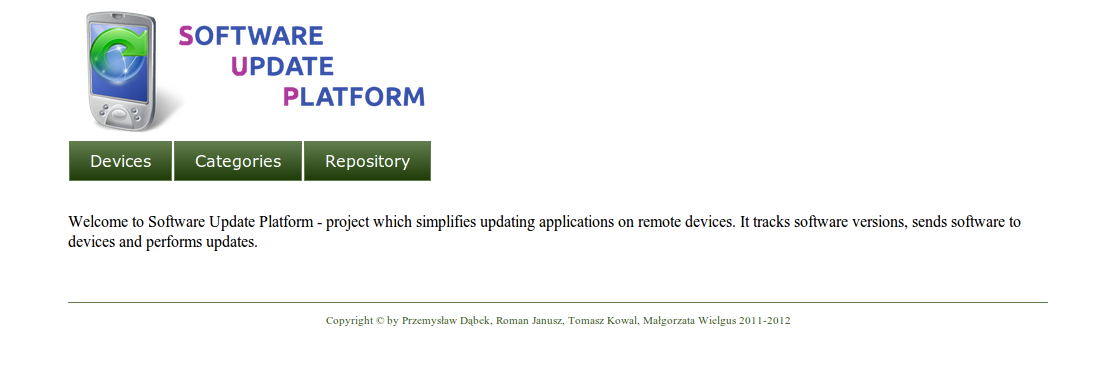
\includegraphics{mainscreen.png}
	}
}

\subsection{Zarządzanie urządzeniami i oprogramowaniem}
\subsubsection{Urządzenia}
Podstrona \emph{Devices} jest odpowiedzialna za zarządzanie urządzeniami zapisanymi w bazie danych. \emph{Filter devices by category} filtruje urządzenia wyłącznie wg danej kategorii; 'pusta' kategoria oznacza wszystkie urządzenia. Poniżej znajduje się lista wszystkich urządzeń zgodnie z ustawionym filtrem kategorii. Dla każdego urządzenia tabela zawiera informację o nazwie, czasie ostatniego połączenia serwera z nim i adresie IP. Po lewej stronie każdego urządzenia w liście jest widoczny checkbox, który jest wykorzystywany przez formularz w sekcji \emph{Enqueue jobs} służący do zlecania aktualizacji oprogramowania. Przycisk \emph{View} po prawej stronie przenosi do podstrony ze szczegółowymi informacjami o danym urządzeniu.

\centerline{
	\scalebox{0.5}{
		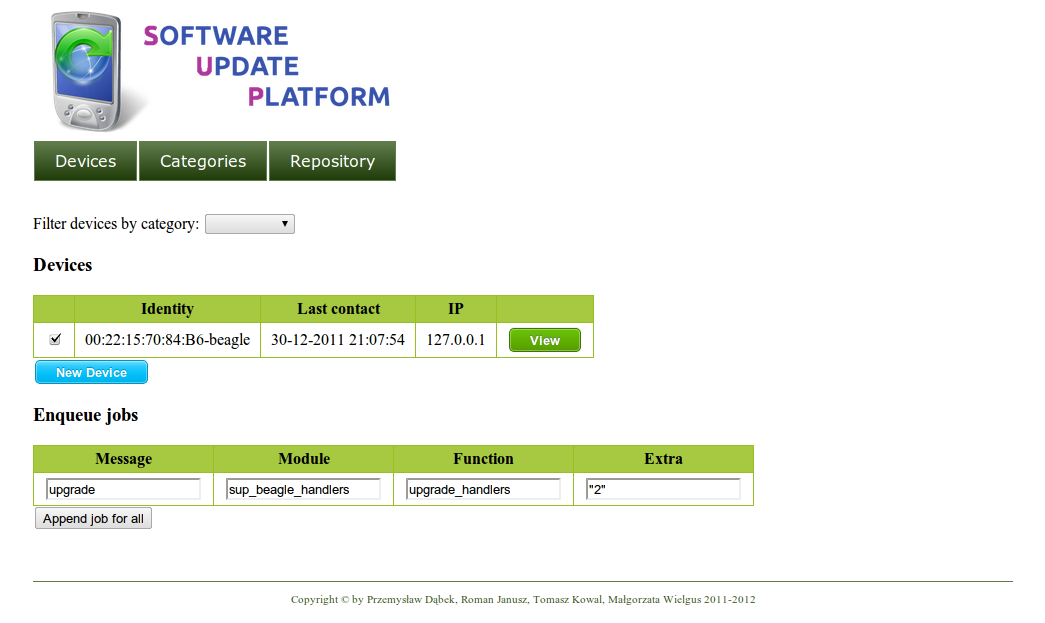
\includegraphics{devices.png}
	}
}

W szczegółowym widoku o urządzeniu można:
\begin{itemize}
\item sprawdzić informację o wersji \emph{release'u}
\item usunąć je z platformy,
\item przypisać do wybranych kategorii,
\item dowiedzieć się o zainstalowanych aplikacjach w release,
\item zlecić zadania do wykonania,
\item obejrzeć historię zakończonych zadań.
\end{itemize}
\clearpage

\centerline{
	\scalebox{0.5}{
		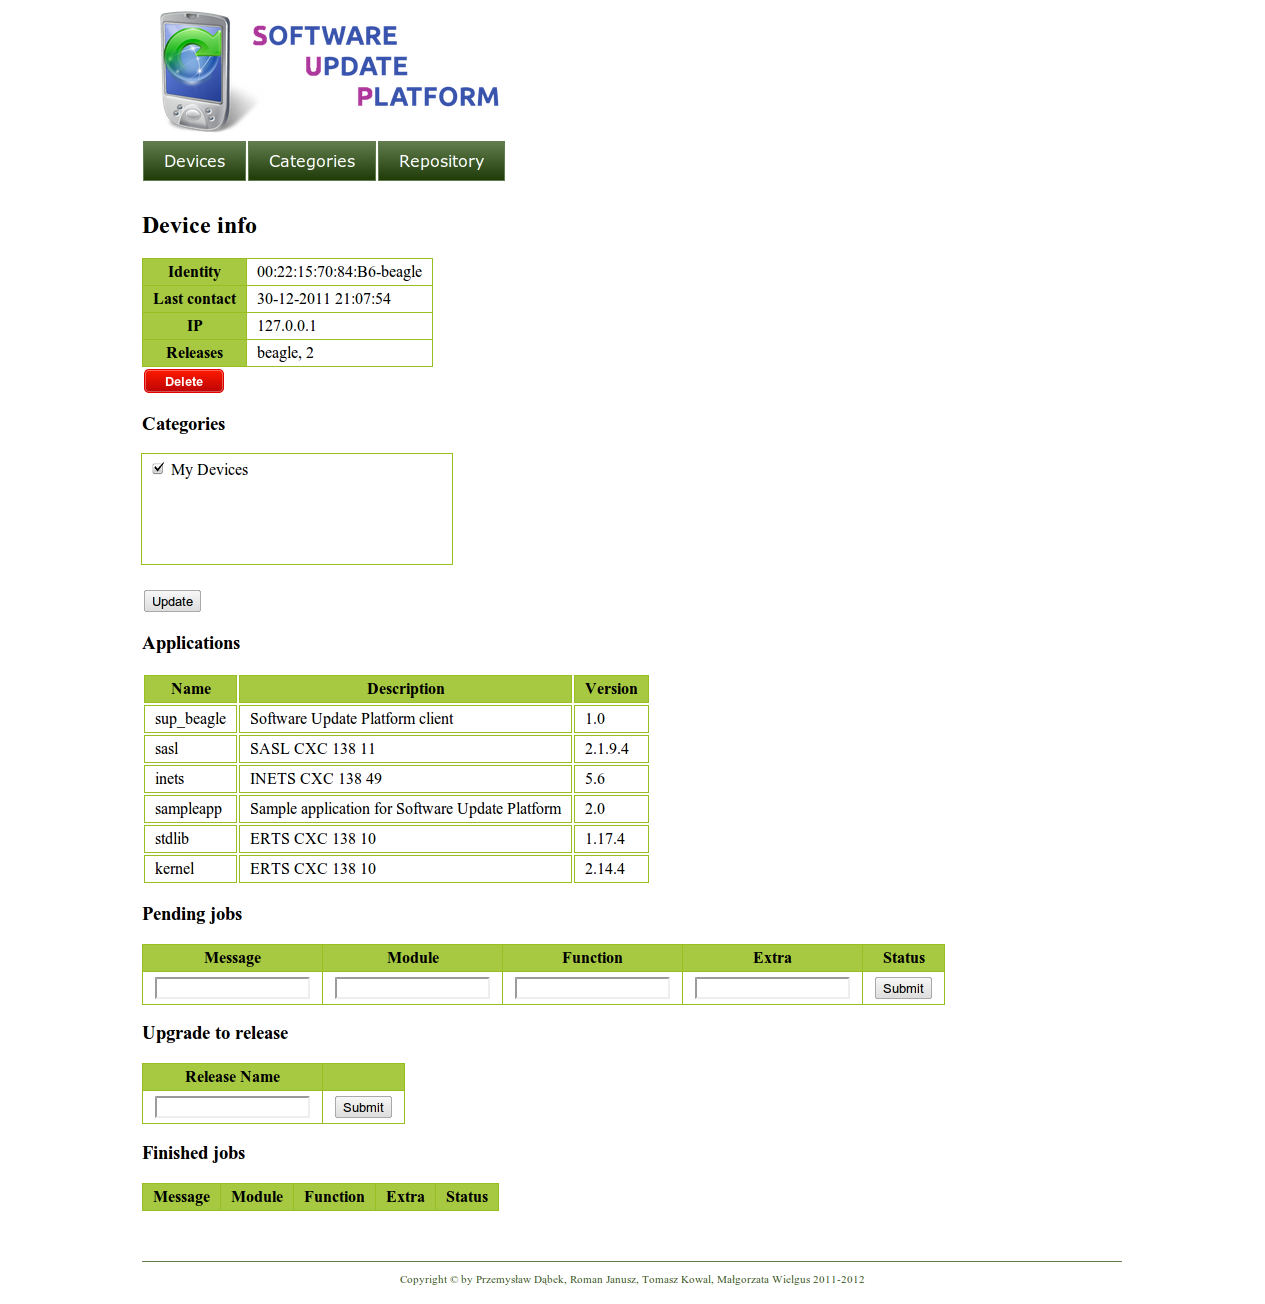
\includegraphics{device.png}
	}
}

\subsubsection{Kategorie}
Podstrona \emph{Categories} jest odpowiedzialna za dodawanie i usuwanie kategorii, do których można przypisać urządzenia. Dla każdej kategorii tabela zawiera informacje o nazwie i ilości urządzeń do niej przyporządkowanych.

\centerline{
	\scalebox{0.5}{
		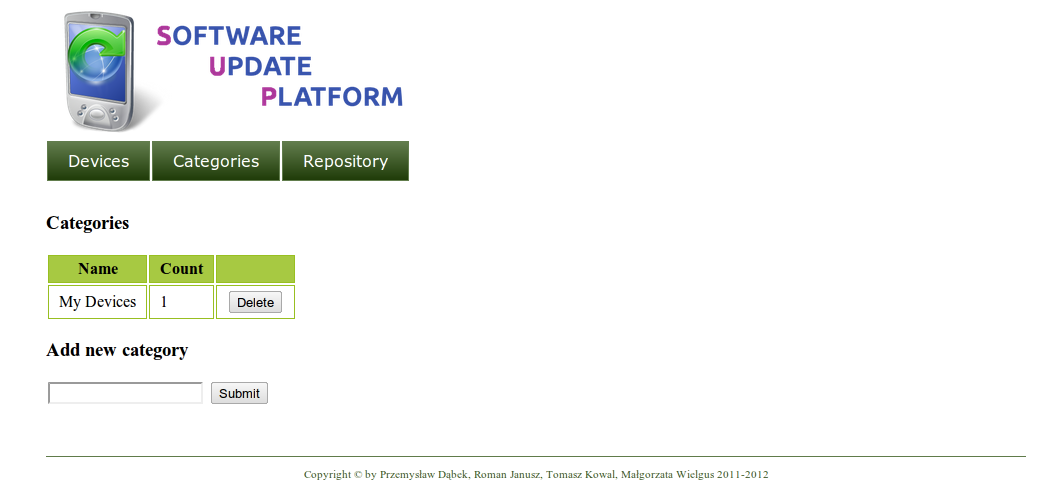
\includegraphics{categories.png}
	}
}

\subsubsection{Repozytorium}
Repozytorium służy do przechowywania wcześniej przygotowanych paczek debianowych. Folder główny, \emph{binary} oraz \emph{source} są dostępnymi lokalizacjami, w których można umieszczać paczki.

\centerline{
	\scalebox{0.5}{
		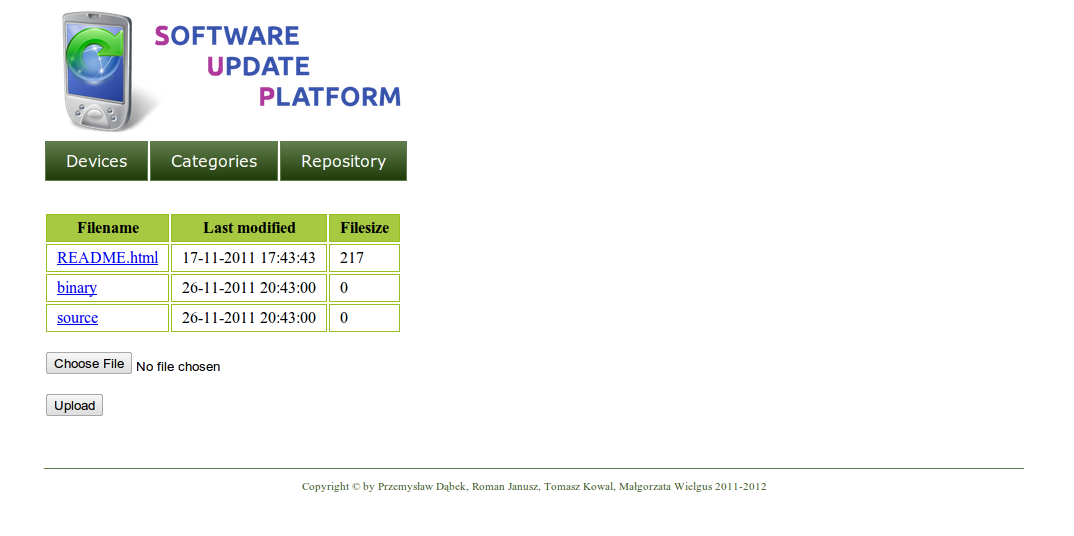
\includegraphics{repository.png}
	}
}

\section{Model rozwoju aplikacji zarządzanej przez platformę}
Platforma do automatycznych aktualizacji zakłada określony wzorzec tworzenia oprogramowania zarządzanego przez platformę. Jest to konieczne ze względu na zależność mechanizmów używanych w systemie (np. paczkowania w pakiety \emph{.deb}).

\subsection{Podstawowe założenia}
Podstawowymi założeniami i ograniczeniami przyjętymi dla modelu rozwoju aplikacji zarządzanej przez platformę są:
\begin{itemize}
\item W systemie używanym do tworzenia oprogramowania musi być obecny Erlang. Od jego wersji i architektury zależy wersja runtime'u wchodzącego w skład wynikowych paczek na urządzenia zdalne. Erlang jest również używany przez większość skryptów dostarczanych wraz z platformą. Dodatkowo, skrypty generujące paczki debiana korzystają z silnika szablonów  erlydtl \url{https://github.com/evanmiller/erlydtl}, który musi być zainstalowany w systemie.
\item W celu tworzenia pakietów .deb konieczna jest obecność w systemie menedżera pakietów dpkg.
\item Fragmentem oprogramowania zarządzanym przez platformę jest erlangowy  release \url{http://www.erlang.org/doc/design_principles/release_structure.html} tworzony zgodnie z wzorcami Erlang OTP \url{http://www.erlang.org/doc/design_principles/users_guide.html}. Zakłada się, że użytkownik platformy tworzący oprogramowanie przez nią zarządzane jest zaznajomiony z wzorcami tworzenia oprogramowania w Erlangu (OTP).
\item Oprogramowanie wdrażane jest na urządzenia zdalne w postaci tzw. węzła wbudowanego (erlang embedded node). Oznacza to wykorzystanie konkretnych mechanizmów instalacji, aktualizacji i uruchamiania węzła. Przez większość czasu są one niewidoczne dla użytkownika, jednak należy o nich pamiętać podczas tworzenia np. paczek aktualizacyjnych.
\item Oprogramowanie w Erlangu tworzone jest z wykorzystaniem narzędzia rebar \url{https://github.com/basho/rebar}. Zakłada się znajomość tego narzędzia przez twórcę oprogramowania zarządzanego przez platformę. Ze względu na niedociągnięcia w standardowej wersji, użyta została  wersja z poprawkami \url{https://github.com/smarkets/rebar}.
\end{itemize}

Szczegóły nt. wyżej wymienionych założeń, ograniczeń i narzędzi opisane są w dalszych częściach dokumentacji.

\subsection{Tworzenie środowiska rozwoju oprogramowania zarządzanego przez platformę}
Platforma udostępnia jako plik archiwum przykładową strukturę katalogów wraz z wykorzystywanymi narzędziami, która może służyć do tworzenia release'u erlangowego zarządzanego przez platformę.

Zawartość środowiska startowego:

\begin{lstlisting}
devenv/
    rebar
    rebar.config
    apps/
        sup_beagle/
            ...
    rel/
        genrelup
    debian/
        debian.config
        templates/
            ...
        makebasedeb
        makeappdeb
        makereldeb
\end{lstlisting}

\subsubsection{rebar}
Plik wykonywalny zawierający narzędzie rebar. W celu łatwiejszego jego użycia można umieścić katalog ze środowiskiem w zmiennej PATH lub stworzyć alias w shellu odwołujący się do tego skryptu.
\subsubsection{rebar.config}
Plik konfiguracyjny rebara. Początkowa zawartość tego pliku jest następująca:
\begin{lstlisting}
{sub_dirs, [
            "rel",
            "apps/sup_beagle"
           ]
}.
\end{lstlisting}
Jak widać, konfiguracja rebara sprowadza się do wylistowania podkatalogów, które mają być przez niego widoczne. Plik ten wymaga edycji podczas dodawania lub usuwania aplikacji \url{http://www.erlang.org/doc/design_principles/applications.html} do release'u erlangowego przez programistę. Przykładowo, dodanie erlangowej aplikacji o nazwie \texttt{sampleapp} wymaga dodania do listy \texttt{sub\_dirs} elementu \texttt{"apps/sampleapp"}.
\subsubsection{apps}
Katalog ten zawiera źródła wszystkich aplikacji erlangowych tworzonych przez programistę, które mają znaleźć się w wynikowym release. Domyślnie katalog ten zawiera źródła aplikacji \texttt{sup\_beagle} będącej klientem platformy automatycznych aktualizacji. Aplikacja ta musi znaleźć się w wynikowym release. Źródła wszystkich innych tworzonych aplikacji należy umieścić w katalogu \texttt{apps}, w podobny sposób jak aplikację \texttt{sup\_beagle} (tj. źródła w podkatalogu src, pliki nagłówkowe w katalogu \texttt{include}, itp.). Dla każdej aplikacji należy również dodać wpis w pliku konfiguracyjnym rebara (patrz wyżej).
\subsubsection{rel}
Ten katalog służy do generacji wynikowych węzłów erlangowych za pomocą rebara (komenda generate - szczegóły w odpowiedniej sekcji dokumentacji). Wygenerowany przez rebara węzeł jest obrazem wynikowego środowiska docelowego zawierającego erlangowy runtime z zestawem skryptów i plików konfiguracyjnych oraz skompilowanym release'm. Środowisko takie stanowi podstawę do generacji paczek debiana, gotowych do instalacji na urządzeniu zdalnym.

Skrypt \texttt{genrelup} służy do tworzenia w węźle docelowym pliku relup \url{http://www.erlang.org/doc/man/relup.html}. Szczegóły jego użycia opisane są w sekcji dotyczącej generowania paczek debiana.
\subsubsection{debian}
Katalog ten zawiera zestaw skryptów oraz plik konfiguracyjny używane do generacji paczek \emph{.deb}. Jest to również katalog, w którym umieszczane będą wygenerowane paczki. Szczegóły nt. użycia skryptów i konfiguracji opisane są w sekcji dotyczącej generacji paczek.

\subsection{Inicjalizacja węzła erlangowego}
Po stworzeniu bazowego środowiska należy zainicjalizować węzeł erlangowy za pomocą rebara. W tym celu należy wejść do katalogu \texttt{rel} i wykonać następującą komendę:
\begin{lstlisting}
../rebar create-node nodeid=id_wezla
\end{lstlisting}

\texttt{id\_węzła} jest dowolnym identyfikatorem docelowego węzła erlangowego. Służy on również m.in. jako nazwa release'u i (domyślnie) stanowi bazową nazwę dla paczek debiana.

Efektem wykonania komendy jest wygenerowanie przez rebara w katalogu \texttt{rel} plików \texttt{reltool.config}, \texttt{sys.config} oraz podkatalogu \texttt{files}.

\subsubsection{reltool.config}

Plik konfigurujący zachowanie komendy \texttt{rebar generate}. Ściślej: konfiguruje zachowanie funkcji z erlangowego pakietu \texttt{reltool} używanego wewnętrznie przez rebara do generacji docelowych release'ów i węzłów.

Wymagana jest edycja tego pliku i dodanie do niego następujących wpisów:
\begin{itemize}
\item wpisanie katalogu z źródłami aplikacji (\texttt{"../apps"}) do listy \texttt{lib\_dirs}
\item wylistowanie wszystkich aplikacji wchodzących w skład release'u o nazwie odpowiadającej id węzła (obowiązkowo należy wylistować aplikację \texttt{sup\_beagle})
\item nadanie release'owi pożądanego numeru wersji
\end{itemize}

Uwaga: dla poprawnego działania skryptów zarządzających w paczkach \emph{.deb} wymagane jest pozostawienie pustego release'u \texttt{start\_clean} oraz opcji \texttt{\{excl\_archive\_filters, [".*"]\}}.

Gotowy plik \texttt{reltool.config} dla release'u o nazwie \texttt{beagle} w wersji 2 zawierającego aplikację \texttt{sampleapp} może wyglądać następująco:
\begin{lstlisting}
{sys, [
       {lib_dirs, ["../apps"]},
       {rel, "beagle", "2",
        [
         kernel,
         stdlib,
         sup_beagle,
         sampleapp
        ]},
       {rel, "start_clean", "",
        [
         kernel,
         stdlib
        ]},
       {boot_rel, "beagle"},
       {profile, embedded},
       {incl_cond, exclude},
       {excl_sys_filters, ["^bin/.*",
                           "^erts.*/bin/(dialyzer|typer)"]},
       {excl_archive_filters, [".*"]},
       {app, sup_beagle, [{incl_cond, include}]},
       {app, sampleapp, [{incl_cond, include}]},
       {app, kernel, [{incl_cond, derived}]},
       {app, stdlib, [{incl_cond, derived}]},
       {app, sasl, [{incl_cond, derived}]},
       {app, inets, [{incl_cond, derived}]}
      ]}.

{target_dir, "beagle"}.

{overlay, [
           {mkdir, "log/sasl"},
           {copy, "files/erl", "\{\{erts_vsn\}\}/bin/erl"},
           {copy, "files/nodetool", "\{\{erts_vsn\}\}/bin/nodetool"},
           {copy, "files/beagle", "bin/beagle"},
           {copy, "files/beagle.cmd", "bin/beagle.cmd"},
           {copy, "files/start_erl.cmd", "bin/start_erl.cmd"},
           {copy, "files/app.config", "etc/app.config"},
           {copy, "files/vm.args", "etc/vm.args"}
          ]}.
\end{lstlisting}
\subsubsection{sys.config}
Plik zawierający domyślną konfigurację release'u, tj. zbiorczą konfigurację aplikacji erlangowych wchodzących w jego skład.

\subsubsection{files}
Katalog zawierający pliki używane przez rebara do generacji węzła wynikowego.

\subsection{Kompilacja i generacja węzła docelowego}
Aby skompilować aplikacje zawarte w docelowym release erlangowym, w głównym katalogu środowiska należy wywołać komendę texttt{./rebar compile}

Po kompilacji można wygenerować węzeł docelowy za pomocą komendy \texttt{./rebar generate} która w katalogu \texttt{rel} stworzy katalog o nazwie takiej jak id węzła zawierający docelowy węzeł erlangowy. Nadaje się on do testowego uruchamiania. Służy do tego skrypt o nazwie takiej, jak id węzła w podkatalogu katalogu \texttt{bin} w wygenerowanym węźle.

\subsubsection{Zachowywanie starych wersji}

W celu generacji plików appup i \texttt{relup} służących do wykonywania upgrade'ów ze starszych wersji release'u, konieczne jest zachowywanie starszych wersji wygenerowanych węzłów docelowych. W tym celu wystarczy zachować katalog z wygenerowanym węzłem w danej wersji pod inną nazwą.

\subsection{Generacja paczek debiana}
Do tworzenia pakietów .deb służy zestaw skryptów w katalogu debian. Przed ich użyciem należy je skonfigurować, używając do tego pliku \texttt{debian.config}. Zawiera on następujące opcje:
\begin{itemize}
\item \texttt{nodename} - nazwa węzła - musi być taka sama jak id węzła użyty podczas inicjalizacji węzła (komenda \texttt{rebar create-node})
\item \texttt{source\_dir} - katalog z wygenerowanym węzłem erlangowym służący jako źródło plików umieszczanych w paczkach debiana.
\item \texttt{target\_root} - katalog systemu docelowego na urządzeniu zdalnym, w którym zainstalowany zostanie wygenerowany węzeł erlangowy
\item \texttt{maintainer} - dane osoby zarządzającej paczkami \emph{.deb} w postaci \emph{Imię Nazwisko <email>}. Dane te zostaną umieszczone w plikach \texttt{control} pakietów debiana (opcja \texttt{Maintainer}).
\item \texttt{description} - opis umieszczany w pliku \texttt{control} pakietu debiana generowanego przez skrypt \texttt{makereldeb} (opcja \texttt{Description})
\end{itemize}
Przykładowa zawartość pliku debian.config dla węzła o nazwie beagle może wyglądać następująco:
\begin{lstlisting}
{nodename, "beagle"}.
{source_dir, "../rel/beagle"}.
{target_root, "/opt/beagle"}.
{maintainer, "Jan Kowalski <jankowalski@gmail.com>"}.
{description, "Sample SUP-managed node for Beagleboard"}.
\end{lstlisting}

\subsubsection{Zarys modelu generacji paczek debiana}
Węzeł erlangowy wygenerowany za pomocą rebara dzielony jest na następujący zestaw pakietów debiana:
\begin{itemize}
\item pakiet bazowy zawierający erlangowy runtime oraz zestaw skryptów stworzonych przez rebara do uruchamiania węzła. Pakiet ten jest zależny od architektury, a jego wersja odpowiada wersji ERTS (Erlang Run-Time System) węzła. Nazwa pakietu bazowego to \texttt{nazwa\_węzła-base}.
\item osobny pakiet dla każdej aplikacji erlangowej wchodzącej w skład release'u. Pakiety te są niezależne od architektury (opcja \texttt{Architecture} w pliku \texttt{control} ma wartość /texttt{all}). Wersja każdego pakietu odpowiada wersji aplikacji. Nazwa pakietu z aplikacją to \texttt{nazwa\_węzła-nazwa\_aplikacji}
\item pakiet główny, zawierający pliki release'u samego w sobie. Pakiet ten jest zależny od pakietu bazowego i pakietów aplikacji. Zależność jest ścisła, tj. wyspecyfikowane są konkretne wersje pakietów zależnych i tylko te mogą być akceptowane podczas instalacji. Nazwa pakietu głównego jest taka sama jak nazwa węzła.
\end{itemize}

Podział na wiele pakietów służy zmniejszeniu ilości danych pobieranych podczas aktualizacji oprogramowania. Nie należy wykonywać żadnych operacji bezpośrednio na pakietach innych niż pakiet główny.

\subsubsection{Obsługa aktualizacji}
Budując pakiety dla kolejnych release'ów należy pamiętać o kilku czynnościach, które należy wykonać przed wygenerowaniem węzła z nową wersją release'u bez których automatyczna aktualizacja może nie działać:
\begin{itemize}
\item należy zawsze zmienić wersję release'u na wyższą w pliku \texttt{reltool.config}. Oczywiście należy również pamiętać o zmienianiu wersji samych aplikacji, które się zmieniły, w ich plikach \emph{.app}.
\item konieczne jest zachowywanie wygenerowanych komendą \texttt{rebar generate} węzłów dla starych wersji release'u (tj. dla tych wersji, z których może być wykonywana aktualizacja).
\item w katalogach źródłowych aplikacji, których wersja się zmieniła należy stworzyć pliki appup \url{http://www.erlang.org/doc/man/appup.html} definiujące sposób aktualizacji pojedynczej aplikacji. W tym celu można posłużyć się komendą \texttt{rebar\ generate-appupps}, jednak należy zważyć na jej ograniczoną funkcjonalność (możliwe jest wyspecyfikowanie tylko jednej starej wersji release'u). Pliki \texttt{appup} są konieczne do wygenerowania pliku \texttt{relup} za pomocą skryptu \texttt{generelup}
\end{itemize}

\subsubsection{genrelup}

Generując zestaw pakietów dla nowej wersji release'u, w celu obsługi aktualizacji należy wygenerować plik \texttt{relup} definiujący sposób aktualizacji release'u na urządzeniu zdalnym, "na żywo" (hot upgrade). Służy do tego skrypt \texttt{genrelup} o następującej składni:
\begin{lstlisting}
genrelup release target_rel_dir:vsn upfrom_rel_dir:vsn,... \
downto_rel_dir:vsn,...
\end{lstlisting}

\begin{itemize}
\item \texttt{release} jest nazwą release'u (identyczna z id węzła)
\item \texttt{target\_rel\_dir:vsn} definiuje katalog z docelowym węzłem wraz z wersją release'u
\item \texttt{upfrom\_rel\_dir:vsn,...} to oddzielana przecinkami lista katalogów z wygenerowanym węzłem oraz wersją releasu, z których może zostać wykonana aktualizacja
\item \texttt{downto\_rel\_dir:vsn,...} to oddzielana przecinkami lista katalogów z wygenerowanym węzłem oraz wersją releasu, do których może zostać wykonany downgrade (downgrade nie jest obsługiwany przez platformę, lecz potencjalnie może być wykonywany ręcznie)

Przykładowe wywołanie skryptu generujące plik relup dla releasu o nazwie \texttt{beagle} w wersji 3 w węźle w katalogu \texttt{beagle-new} dla starych wersji release'u 1 i 2 zawartych w węźle wygenerowanym w katalogu \texttt{beagle-old}:
\begin{lstlisting}
genrelup beagle beagle-new:3 beagle-old:1,beagle-old:2
\end{lstlisting}
\subsubsection{Tworzenie plików \emph{.deb}}
Do generacji finalnych paczek służą skrypty \texttt{makebasedeb},\texttt{makeappdeb} oraz \texttt{makereldeb}. Skrypty te zapisują wygenerowane pakiety w katalogu \texttt{debian}.
\subsubsection{makebasedeb}
Skrypt tworzący pakiet bazowy. Nie wymaga żadnych parametrów.
\subsubsection{makeappdeb}
Skrypt tworzący pakiet dla danej aplikacji erlangowej. Składnia:
\begin{lstlisting}
makeappdeb nazwa_aplikacji [wersja_aplikacji]
\end{lstlisting}
Jeśli węzeł zawiera tylko jedną wersję danej aplikacji, specyfikowanie wersji nie jest konieczne.
\subsubsection{makereldeb}
Skrypt służący do generacji pakietu głównego dla release'u. Składnia:
\begin{lstlisting}
makereldeb wersja_releasu
\end{lstlisting}

\end{itemize}


\end{document}
